\documentclass{article}
%encoding
%--------------------------------------
\usepackage[utf8]{inputenc}
\usepackage[T1]{fontenc}
%--------------------------------------
 
%German-specific commands
%--------------------------------------
\usepackage[ngerman]{babel}
\usepackage{csquotes}
%--------------------------------------
 
%Pictures
%--------------------------------------
\usepackage{graphicx}
\graphicspath{ {./Pictures/} }
\usepackage{tikz}
\usepackage{subcaption}
\usepackage{float}
\usepackage{wrapfig}
%--------------------------------------

%math
%--------------------------------------
\usepackage{amsmath}
\usepackage{amssymb}
\usepackage{amsfonts}
%--------------------------------------

%Frames
%--------------------------------------
\usepackage{framed}

%Own math commands
%--------------------------------------
\newcommand{\abs}[1]{\lvert#1\rvert}

%Colors
%--------------------------------------
\usepackage{xcolor}
\definecolor{blue-violet}{rgb}{0.54, 0.17, 0.89}
\definecolor{codegreen}{rgb}{0,0.6,0}
\definecolor{codegray}{rgb}{0.5,0.5,0.5}
\definecolor{codepurple}{rgb}{0.58,0,0.82}
\definecolor{backcolour}{rgb}{0.95,0.95,0.92}

%--------------------------------------
%\usepackage{multicol}
\usepackage{paracol}
\usepackage[shortlabels]{enumitem}

%Aufgaben
%--------------------------------------
\usepackage{amsthm}
\newtheorem{aufgabe}{Aufgabe}[section]
\newtheorem{definition}{Definition}[section]
\newtheorem{beispiel}{Beispiel}[section]
%--------------------------------------

%Listings
%--------------------------------------
\usepackage{ulem}
\usepackage{listings}
 
\lstdefinestyle{mystyle}{
    backgroundcolor=\color{backcolour},   
    commentstyle=\color{codegreen},
    keywordstyle=\color{magenta},
    numberstyle=\tiny\color{codegray},
    stringstyle=\color{codepurple},
    basicstyle=\ttfamily\footnotesize,
    breakatwhitespace=false,         
    breaklines=true,                 
    captionpos=b,                    
    keepspaces=true,                 
    numbers=left,                    
    numbersep=5pt,                  
    showspaces=false,                
    showstringspaces=false,
    showtabs=false,                  
    tabsize=2,
}
 
\lstset{style=mystyle,moredelim=[is][\sout]{|}{|}}
%--------------------------------------



\title{Einführung in die Automatentheorie - Konzeption}
\author{Alexandra Maximova}
\date{26. Oktober 2020}

\begin{document}

\maketitle
\section{Rahmenbedingungen und Vorwissen}
Diese Lektion wird im Rahmen vom Einführungspraktikum an der Kantonsschule Menzingen gehalten und richtet sich an SuS des vierten Jahres am Kurzzeitgymnasium, die das Ergänzungsfach Informatik absolvieren.

In dieser Lektion geht es darum, endliche Automaten und wichtige Grundbegriffe einzuführen, so dass in den nächsten Lektionen darauf aufgebaut werden kann.

\section{Stoffanalyse}
\begin{figure}[H]
\centering
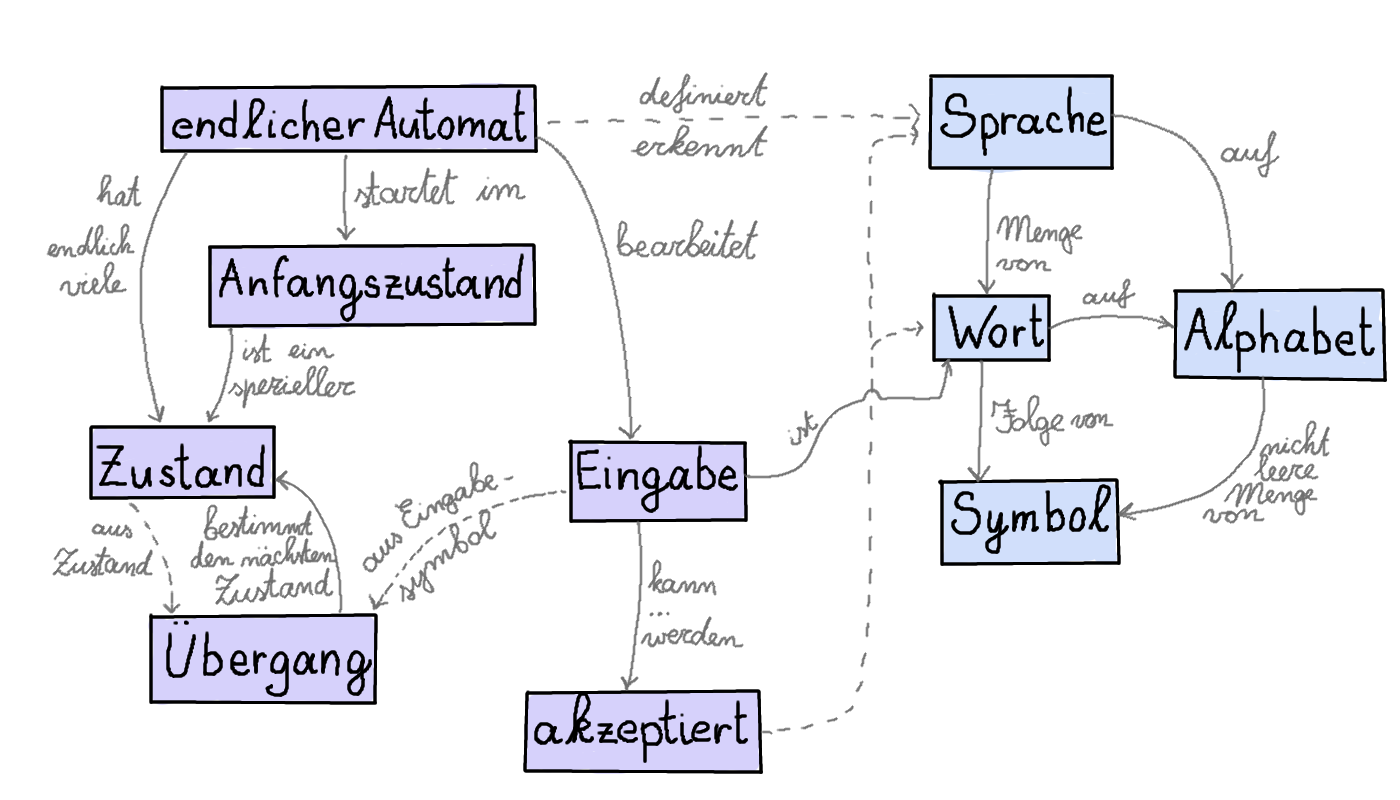
\includegraphics[width=\linewidth]{Pictures/ConceptMap.png}
\end{figure}

Ein \textbf{endlicher Automat} ist ein Programm ohne Variablen, welches eine \textbf{Eingabe} einmal von links nach rechts liest und in Abhängigkeit nur vom aktuell eingelesenen \textbf{Symbol} und vom aktuellen \textbf{Zustand} ins nächste Zustand \textbf{übergeht}. Das Programm startet die Ausführung im \textbf{Anfangszustand} und bestimmt den jeweils nächsten Zustand in Abhängigkeit vom eingelesenen Symbol und vom Zustand. Wenn der Automat nach der Bearbeitung einer Eingabe in einem der speziellen \textbf{akzeptierenden Zustände} endet, dann sagt man, dass der Automat diese Eingabe akzeptiert.

Damit wir einen endlichen Automat formaler und genauer definieren können, brauchen wir folgende Begriffe.

Ein \textbf{Alphabet} ist eine nichtleere Menge von Symbolen. Ein \textbf{Wort} auf einem Alphabet ist eine (möglicherweise leere) Folge von Symbolen aus dem Alphabet. Eine (formale) \textbf{Sprache} ist eine (möglicherweise leere) Menge von Wörter.

Formal können wir nun den endlichen Automaten als Quintupel \(M = (Q, \Sigma, \delta, q_0, F)\) beschreiben, wobei \(Q\) eine endliche Menge der \textbf{Zustände}, \(Sigma\) das \textbf{Eingabealphabet}, \(\delta: Q \times \Sigma \rightarrow Q\) die \textbf{Übergangsfunktion}, \(q_0 \in Q \) der \textbf{Anfangszustand} und \(F \subseteq Q\) die Menge der \textbf{akzeptierenden Zustände} sind.

Ein endlicher Automat bearbeitet Wörter auf \(\Sigma\). Er startet im Zustand \(q_0\) und liest von links nach rechts die Eingabe Symbol für Symbol. Die Übergangsfunktion \(\delta\) beschreibt, wie er dabei von einem Zustand zum anderen abhängig vom eingelesenen Symbol übergeht. Wenn der Automat sich nach der Ausführung auf der Eingabe \(w\) in einem Zustand aus \(F\) befindet, dann sagt man, dass der Automat \(w\) \textbf{akzeptiert}. Die Menge aller Wörter, die von einem Automaten akzeptiert werden, kann man als Sprache anschauen.

\section{Lernziele}
\paragraph{Leitidee}
Jeder von uns hat in der Tasche einen Computer, der mächtiger ist als der, der die Menschen auf den Mond brachte. Diese Computer können über Netz noch mehr Rechenkapazität beanspruchen. Wir haben das Gefühl, wir können alles berechnen, was wir uns nur vorstellen können. Aber lässt sich tatsächlich alles berechnen? Und was bedeutet es überhaupt, etwas zu berechnen?

Endliche Automaten bieten einen spannenden Einstieg in die mathematische Modellierung von Berechnungsarten. Sie sind an konkreten alltäglichen Objekten angelehnt, wie Aufzüge und Getränkeautomaten, und lassen sich elegant mathematisch formulieren. Die SuS sehen, wie alltägliche Objekte abstrahiert und formalisiert werden, und welche Erkenntnisse über die Existenz und Grösse von Automaten sie aus einer sauberen Formulierung gewinnen können.

\paragraph{Dispositionsziele}
\begin{itemize}
\item Die Abstraktionsfähigkeiten der SuS werden gestärkt. Bei einer Problemstellung konzentrieren sich die SuS auf das Wesentliche und können unwichtige Details ignorieren.
\item Die SuS schauen Automaten mit anderen Augen an. Wenn sie beim Kaffeeautomaten eine heisse Schokolade bestellen, denken sie während der Wartezeit, wie viele Zustände so ein Automat haben könnte.
\end{itemize}

\paragraph{Operationalisierte Lernziele}
\begin{itemize}
\item Die SuS zeichnen einen in Worten beschriebenen Alltagsautomaten, wie z.B. ein Getränkeautomat, ein Parkautomat, ein Aufzug, usw. Dabei achten die SuS, dass
	\begin{itemize}
		\item der Anfangszustand gekennzeichnet ist
		\item die akzeptierende Zustände markiert sind
		\item aus jedem Zustand gibt es für jedes in der Eingabe vorkommendes Symbol einen Pfeil zu einem anderen Zustand.
	\end{itemize}
\item Die SuS beschreiben in Worten die Funktionsweise von einem als Diagramm gegebenen Alltagsautomaten.
\item Gegeben ein Diagramm von einem Automaten und eine Eingabe, die SuS sagen, ob die Eingabe akzeptiert wird oder nicht.
\item Gegeben die formale Beschreibung von einem endlichen Automaten, wobei die Übergangsfunktion in tabellarischen Form gegeben wird, zeichnen die SuS das dazugehörige Diagramm.
\item Gegeben einen Automaten als Diagramm, die SuS beschreiben ihn formal als Quintupel. Die Übergangsfunktion schreiben die SuS in tabellarischer Form auf.
\end{itemize}

\section{Informativer Unterrichtseinstieg}

In dieser Lektion werden wir herausfinden, was Aufzüge, Getränkeautomaten, Ampelschalter und Backöfen gemeinsam haben und wie wir solche Maschinen, auch \textbf{endliche Automaten} genannt, mathematisch modellieren können.

In der ersten Stunde werden wir uns mit dem Konzept von Automat vertraut machen, indem wir einige davon zuerst zusammen und dann in Gruppen entwerfen.

In der zweiten Stunde werden wir versuchen, diesen Begriff formal und mathematisch zu formulieren. Eine mathematische Formulierung erlaubt uns, ein Objekt genau und eindeutig zu definieren und seine Eigenschaften zu analysieren, Aussagen darüber zu machen und diese zu beweisen.

Nehmen wir zum Beispiel einen einfachen Kaffeeautomaten. Dieser Automat verkauft für einen Franken eine Tasse Kaffee oder eine Tasse heisse Schokolade. Der Automat akzeptiert nur 1CHF Münzen und hat zwei Knöpfe: Einen Knopf für Kaffee, einen Knopf für heisse Schokolade. Die Anweisungen für den Benutzer lauten:

\begin{minipage}{0.4\linewidth}
\begin{enumerate}
\item Werfe eine 1CHF Münze.
\item Drücke die Taste "Kaffee" oder die Taste "heisse Schokolade".
\item Nehme deinen Becher aus der Maschine.
\end{enumerate}
\end{minipage} \hfill
\begin{minipage}{0.6\linewidth}
\begin{figure}[H]
\centering
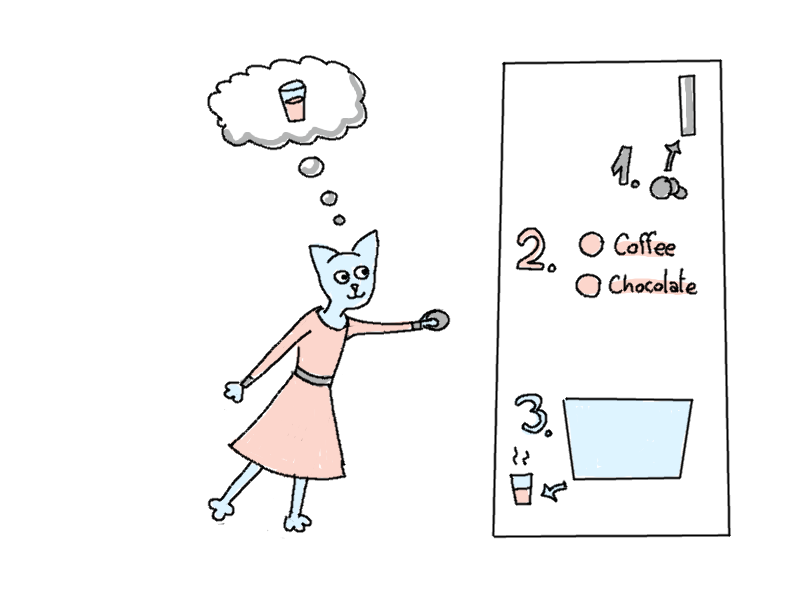
\includegraphics[width=\linewidth]{Pictures/image.png}
\end{figure}
\end{minipage}



Wie würden wir eine solche Maschine Programmieren? Wie muss sich die Maschine verhalten?

Am Anfang wartet der Automat, dass der Benutzer eine Münze einwirft. Wenn eine 1CHF Münze kommt, dann wartet der Automat, welcher Knopf gedruckt wird. Nachdem ein Knopf selektiert wurde, bereitet der Automat das Getränk vor, lässt es unten erscheinen und wartet darauf, dass der Benutzer sein Getränk herausnimmt. Jetzt kann der Automat wieder auf eine Münze warten. Schematisch können wir diesen Verlauf so darstellen.

\begin{figure}[H]
\centering
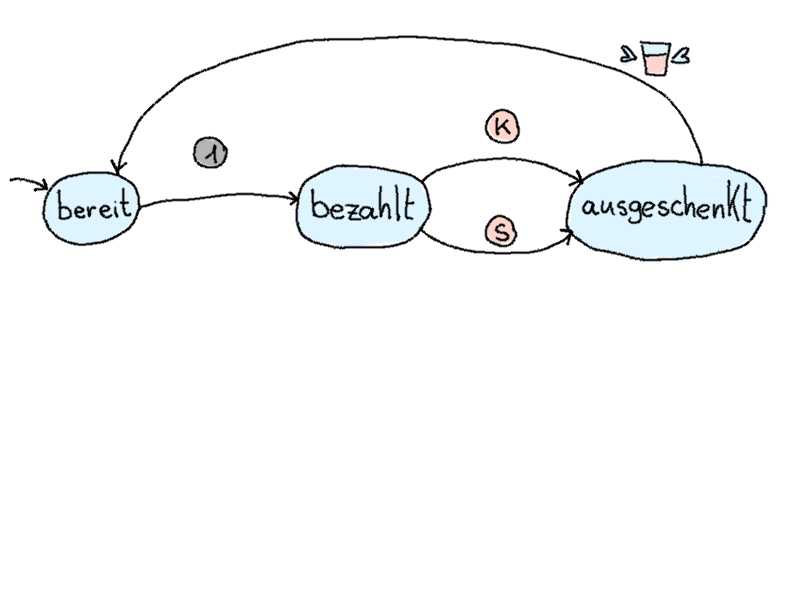
\includegraphics[width=0.7\linewidth]{Pictures/Getraenkeautomat1.png}
\end{figure}

Die hellblaue Kreise stellen die \textbf{Zustände} des Automates dar. Im Zustand \texttt{bereit} wartet der Automat, dass eine Münze eingeworfen wird. Wenn eine Münze eintrifft (kleiner grauer Kreis mit einer '1' über dem Pfeil nach \texttt{bezahlt}), geht der Automat in den nächsten Zustand über. Im Zustand \texttt{bezahlt} wartet der Automat, bis einer der zwei Knöpfe betätigt wird. Wenn der Knopf Kaffee (kleiner roter Kreis mit 'K') oder der Knopf Schokolade (kleiner roter Kreis mit 'S') gedrukt wird, dann bereitet der Automat das entsprechende Getränk und geht in den Zustand \texttt{ausgeschenkt} über. Im Zustand \texttt{ausgeschenkt} wartet der Automat, bis das Getränk verschwindet. Dann geht er wieder in den Zustand \texttt{bereit} über und wartet wieder auf die Münze.

Die kleinen Symbole auf den Pfeilen (
\includegraphics[width=20px]{Pictures/Muenze.png}, 
\includegraphics[width=20px]{Pictures/Kaffee.png}, 
\includegraphics[width=20px]{Pictures/Schoggi.png}, 
\includegraphics[width=20px]{Pictures/Becher.png}) stellen die \textbf{Eingabe} dar. Eine Eingabe ist etwas, was der Automat von aussen erhält. In diesem Fall, zur Eingabe gehören all die erwarteten und möglichen Aktionen vom Benutzer: Münzeneinwurf, Knopf Drücken, Becher Entnehmen.

Wie soll der Automat reagieren, wenn der Benutzer die Anweisungen nicht aufmerksam gelesen hat, und eine Eingabe zur falschen Zeit macht? Wenn der Benutzer, zum Beispiel, den Knopf 'Kaffee' betätigt, bevor er die Münze eingeworfen hat? Oder vergisst, den Becher zu entnehmen und schon die nächste Münze wirft? Diese Reaktionen auf 'Fehler' müssen im Automaten auch programmiert werden. Wir müssen das Diagramm so erweitern, dass aus jedem Zustand für jede mögliche Eingabe ein Pfeil zu einem (möglicherweise selben) Zustand führt.

Der einfache Kaffeeautomat aus unserem Beispiel ist ganz nett und gibt alle überflüssigen Münzen zurück. Um dieses Verhalten zu programmieren, brauchen wir noch zwei weitere Zustände: \texttt{rückgabe} und \texttt{rückgabe2}.
Knöpfe, die zur falschen Zeit gedrückt werden, werden ignoriert.

\begin{figure}[H]
\centering
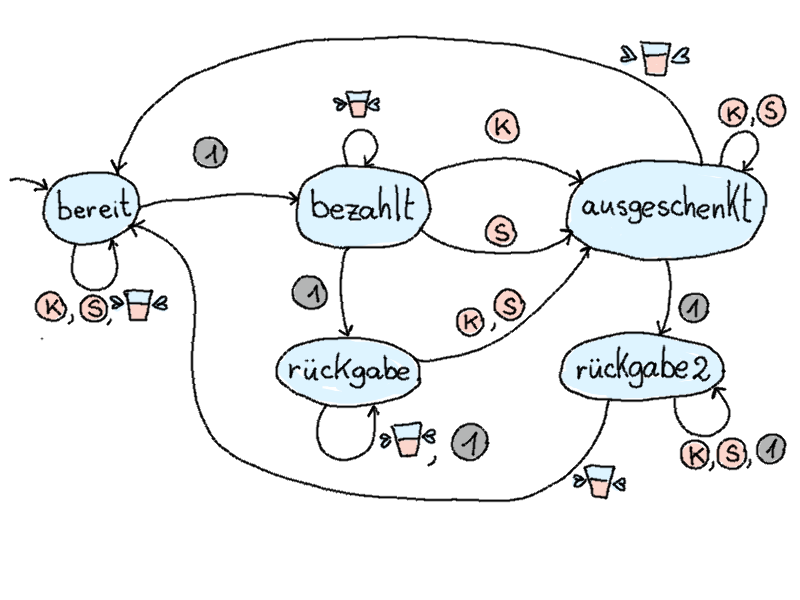
\includegraphics[width=\linewidth]{Pictures/Getraenkeautomat.png}
\end{figure}

In unserem Diagramm haben wir jetzt alle Zustände gezeichnet und für jeden Eingabesymbol haben wir aus jedem Zustand einen Pfeil gezeichnet.  Das sind aber noch nicht alle Informationen, die wir brauchen, um die Funktionalität vom Kaffeeautomaten zu beschreiben. Wir müssen noch definieren, in welchem Zustand der Automat ist, wenn er zum ersten Mal eingeschaltet wird. Dieser spezielle Zustand nennen wir \textbf{Anfangszustand} und kennzeichnen ihn auf dem Diagramm mit einem kurzen Pfeil aus dem nichts. Der Zustand \texttt{bereit} ist bereits als Anfangszustand gekennzeichnet.

Neben dem Anfangszustand, wird in Automaten auch eine andere Art von speziellen Zuständen hervorgehoben, und zwar die, wo eine korrekte Eingabe endet. Im Fall von unserem Kaffeeautomaten, eine korrekte Eingabe ist 
\includegraphics[width=20px]{Pictures/Muenze.png} (Münze werfen), 
\includegraphics[width=20px]{Pictures/Kaffee.png} ('Kaffee' wählen), 
\includegraphics[width=20px]{Pictures/Becher.png} (Becher nehmen). Nach der Bearbeitung dieser Eingabe befindet sich der Automat im Zustand \texttt{bereit}. Solche Zustände nennen wir \textbf{akzeptierende Zustände}. Auf dem Diagramm markiert man sie üblicherweise mit einem doppelten Kreis.

\section{Literatur}
Bei der Vorbereitung vom Skript und Unterricht wurde das Buch "Formale Sprachen" von J. Hromkovic verwendet.

\end{document}